\documentclass{report}

\usepackage{textcomp}
\usepackage{graphicx}
\usepackage{fancyhdr}
\usepackage{subcaption}
\usepackage{multicol}
\usepackage{outlines}
%===================================
\newcommand{\classinfo}{{\bf RHEL LABS \\ Week 05}\\{\it CIT 218}\\{Chaz Davis}}
\newcommand{\semester}{BCTC \\ Spring 2020}
%===================================
\newcommand{\mysection}[1]{\section*{#1}}
\newcommand{\mysubsection}[2]{\textbf{\romannumeral #1) #2}}
%===================================
\setlength{\headheight}{15.2pt}
\pagestyle{fancy}
\fancyhf{}
\lhead{ \fancyplain{}{Chaz Davis} }
\rhead{ \fancyplain{}{\today} }
\cfoot{ \fancyplain{}{\thepage} }
\renewcommand{\headrulewidth}{0.5pt}
\renewcommand{\footrulewidth}{0pt}

%===================================
\title{\classinfo}
\author{\semester}
\date{\today}

%===================================

\begin{document}

\maketitle

%===================================
\mysection{\textbf{Questions}}

\mysubsection{1}{After completing the 11.2. Practice: Create a file in the /mnt/public directory named 
firstname\_lastname. List the files of the directory. Provide the output.}\\
I logged into Desktop1 and mount the directories. In order to gain access to
{\scriptsize{\verb$/mnt/public$}\normalsize}  I logged in through ssh as
{\scriptsize{\verb$ldapuser1@localhost$}\normalsize} and ran the
command {\scriptsize{\verb$touch Chaz_Davis$}\normalsize} and finally, the
command {\scriptsize{\verb$ls -l$}\normalsize} to see the output
in a list format, of which you can see in the screenshot in
Fig.~\ref{Wk05}\subref{Wk05Q01} Pg.~\pageref{Wk05}.

\noindent\mysubsection{2}{After completing the 11.4. Practice: Create a file in the /shares/docs directory named 
firstname\_lastname. List the files of the directory. Provide the output.}\\
I logged into desktop1 and downloaded and created the map files for autofs. I
the logged in as {\scriptsize{\verb$ldapuser1@localhost$}\normalsize} and
created the file {\scriptsize{\verb$Chaz_Davis$}\normalsize} and listed the
docs directory with the command {\scriptsize{\verb$ls -l$}\normalsize}. You can
see the output in Fig.~\ref{Wk05}~\subref{Wk05Q02} 
on Pg.~\pageref{Wk05}.

\noindent\mysubsection{3}{After completing the 12.2. Practice: Create a file in
the /shares/docs directory named firstname\_lastname. List the files of the
directory. Provide the output.}\\
This was the same as the last example, I assumed you wanted me to create the
file in and list the {\scriptsize{\verb$~/work$}\normalsize} directory. So,
that's what I did. The output can be seen in Fig.~\ref{Wk05}\subref{Wk05Q03} on
Pg.~\pageref{Wk05}.




\begin{figure}[!h]\centering
  \subfloat[Public directory listing of filesJ]{\label{Wk05Q01}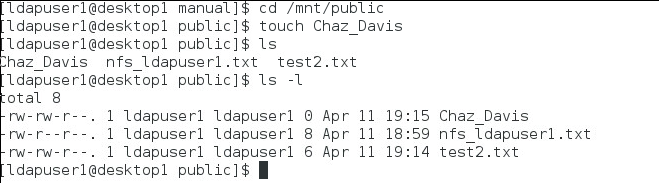
\includegraphics[width=.45\linewidth]{Figures/Q01.png}}\hfill
  \subfloat[docs Directory listing of files]{\label{Wk05Q02}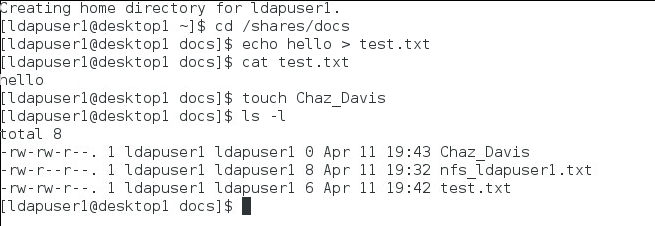
\includegraphics[width=.45\linewidth]{Figures/Q02.png}}\par 
\subfloat[work Directory chapter 12]{\label{Wk05Q03}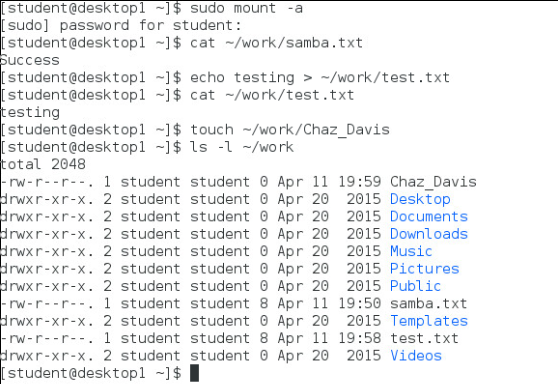
\includegraphics[width=.45\linewidth]{Figures/Q03.png}}
\caption{Screenshots for Chapters 11 and 12 labs}\label{Wk05}
\end{figure}




%===================================

\end{document}
